\documentclass[12pt,a4paper]{article}
 
\usepackage{float}
%für feststellen der figures und tables [H] dranschreiben
\usepackage{units}
%wird so benutzt: 
%\unit[value/Zahl]{dimension/Einheit} oder 
%\unitfrac[value/Zahl]{dimension/Einheit num/Zähler}{dimension/Einheit denum/Nenner} oder
%\nicefrac[fontcommand/Schriftart]{dimension/Einheit num/Zähler}{dimension/Einheit denum/Nenner}
\usepackage[left=2cm,right=2cm,top=2cm,bottom=2cm]{geometry}
\usepackage[utf8]{inputenc}
\usepackage[T1]{fontenc}
\usepackage{lmodern}
\usepackage[ngerman]{babel}
\usepackage{amsmath}
\usepackage{graphicx}
 
\title{Versuch AP4\\ Inelastische Streuung -\\ Das Franck-Hertz-Experiment}
\author{Frederik Strothmann, Henrik Jürgens}
\date{\today}
%es dürfen niemals zwei überschriften direkt übereinander stehen, also immer mindestens in einem satz was sinnvolles unter jede überschrift schreiben. (bei den versuchen z.B. das versuchsziel) 
\begin{document}
%deckblatt erstellen.
\maketitle
\newpage
\tableofcontents
\newpage
\section{Einleitung}
%einleitung zu dem experiment.
%es muss hier auf die einstellungen, die vor dem versuch gemacht werden eingegangen werden oder auf eine anleitung dazu verwiesen werden.
Beim diesem Versuch wird ein Experiment von Franck und Hertz aus dem Jahre 1914 wiederholt. Wir werden untersuchen, dass Quecksilberatome bei inelastischen Stößen mit Elektronen Energie aufnehmen können, wenn diese dem Energieunterschied zweier Anregungsniveaus des Quecksilbers entspricht. Dieses Experiment hatte eine große historische Bedeutung, weil damit -- neben der Emission diskreter Spektrallinien -- gezeigt werden konnte, dass Atome nur diskrete Energiewerte annehmen können. Auch in der heutigen Physik spielen inelastische Streuexperimente, z.B. von Elektronen an Kernen, Protonen und Neutronen, eine wesentliche Rolle, da sie Aufschluß über die innere Struktur der Materie vermitteln. Neben der Anregung von Hg-Atomen wird in diesem Versuch ebenfalls die Anregung von Neonatomen beobachtet. (vgl. Zielsetzung http://www.atlas.uni-wuppertal.de/$\sim$kind/ap22ap4neu.pdf)
\section{Verwendete Materialien}
%immer eine skizze oder ein foto einfügen und die geräte und materialien !nummerieren! und z.b. eine legende dazu schreiben.
%falls wir am anfang des versuches noch nicht wissen, was wir alles brauchen, dann wenn möglich erst am ende ein großes foto von den verwendeten materialien machen!
%-------------------------------------------------------------------------------------------
%ab hier für jeden versuchsteil einzeln und falls doch noch welche materialien hinzugenommen werden immer im versuchsaufbau erwähnen!

\begin{figure}[H] 
  \centering
    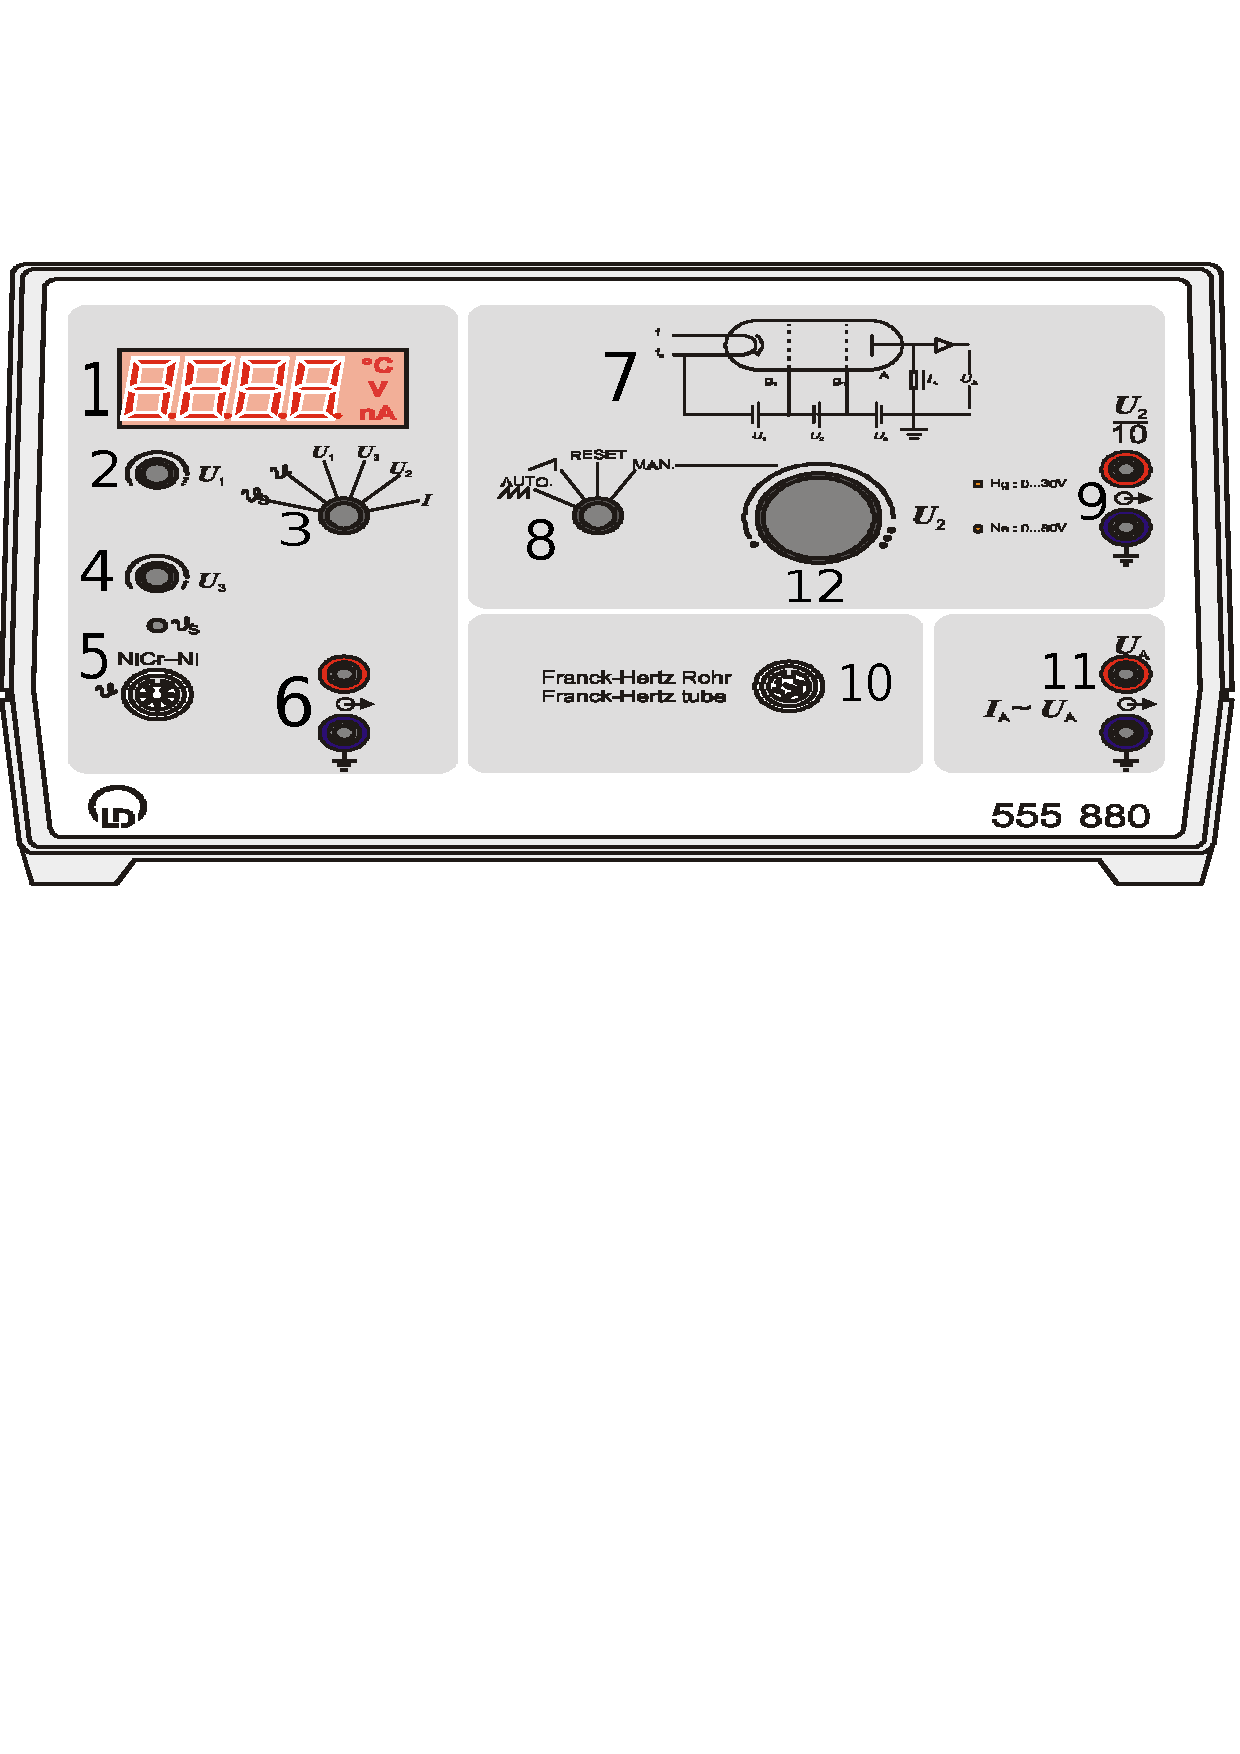
\includegraphics[trim = 0mm 145mm 0mm 40mm, clip, scale = 0.7]{aufbau.pdf}
  	\caption[Abbildung des Franck-Hertz Betriebsgerätes]{Abbildung des Franck-Hertz Betriebsgerätes\footnotemark}
  \label{fig:abb_versuch_3}
\end{figure}
\footnotetext{Abbildung entnommen von http://www.atlas.uni-wuppertal.de/\~kind/franck-hertz-555880d.pdf Seite 1 am 20.09.2014}

\begin{enumerate}
\item	Digitalanzeige 

\item	Spannungsteller für U$_1$

\item	Messgrößeneinstellung

\item	Spannungsteller für U$_3$

\item	5-polige DIN-Buchse, zum Anschluss des Temperaturfühlers

\item	Analogausgang für die gewählte Messgröße

\item	Schaltskizze 

\item	Schalter für die Betriebsart

\item	Analogausgang $\frac{\text{U}_2}{10}$ 

\item	7-poliger DIN-Buchse zum Anschluss des Hg- oder Ne-Franck-Hertz-Rohres.

\item	Analogausgang von U$_\text{A}$

\item	Spannungsteller für U$_2$
\end{enumerate}

\section{Franck-Hertz Versuch für Quecksilber}
%hier am besten kurz das ziel dieses versuchsteiles ansprechen, damit wir keine zwei überschriften übereinander haben!
%bei schwierigeren versuchen kann auch der theoretische hintergrund erläutert werden. (mit formeln, herleitungen und erklärungen)
Ziel der Messung ist es die Franck-Hertz-Kurve für Quecksilber aufzunehmen und aus ihr die Energiedifferenz zwischen Grund- und angeregtem Zustand zu bestimmen, sowie die Kontaktpotentialdifferenz.

\subsection{Versuchsaufbau}
%skizze zum versuchsaufbau soll hier rein, foto geht auch aber es muss erklärt werden wie das ganze funktioniert und nochmal auf spezielle einstellungen eingegangen werden! z.b. welche knöpfe wir an unseren geräten für die messung verdreht haben.
\subsection{Versuchsdurchführung}
%hier soll hauptsächlich rein was wir machen, warum wir das machen und mit welchem ziel.
%es ist wichtig präzize zu erklären wie wir bei dem versuch vorgegangen sind und was wir tuen mussten.
Zuerst muss die Franck-Hertz Röhre (Quecksilber) vorgeheizt werden (die Betriebstemperatur von 175$^{\circ}$ konnte an unserem Gerät nicht verstellt werden), $\frac{U_2}{10}$ (Kanal 1 des Oszilloskops := X-Achse) und $U_A$ (Kanal 2 des Oszilloskops := Y-Achse) an das Oszilloskop angeschlossen werden und die Franck-Hertz Kurve mit der Sägezahnspannung konfiguriert werden. Dazu können die Saugspannung $U_1$ und die Bremsspannung $U_3$ am Franck-Hertz Betriebsgerät verdreht, sowie am Oszilloskop die Auflösung in X- und Y-Richtung und die Verschiebung der Kurve auf der X- und Y-Achse eingestellt werden. Sobald die Franck-Hertz Kurve am Oszilloskop gut zu erkennen ist, kann das Franck-Hertz Betriebsgerät auf den manuellen Modus umgestellt werden. Nun kann die Kurve von Hand durch verändern der Beschleunigungsspannung $U_2$ durchgefahren und einige Messerte aufgenommen werden. Danach werden zusätzlich die genauen Maxima ausgemessen um später die Anregungsspannung bzw. Anregungsenergie aus dem Mittelwert der Differenzspannungen $U_{\Delta}$ (zwischen zwei nebeneinander liegenden Maxima) zu bestimmen.
Zum Schluss wollen wir die Kontaktpotentialdifferenz zwischen Anode und Kathode bestimmen.
Die Beschleunigungsspannung bis zum ersten Maximum ist dafür gleichzusetzen mit der Anregungsspannung der Quecksilberatome und der Kontaktpotentialdifferenz zwischen Anode und Kathode.
\subsection{Verwendete Formeln}
%es kann eine legende angefertigt werden aber die selbstverständlichen buchstaben müssen nicht extra erklärt werden.
%hier kommen mit knappen erklärungen nur die verwendeten formeln, sowie die zugehörige Fehlerrechnung rein.
Die Differenzspannung $U_{\Delta}$ wird aus der Potentialdifferenz zweier nebeneinander liegender Maxima bestimmt:
\begin{align}
U_{\Delta} = U_{max1}-U_{max2}
\label{eqn:u_d}
\end{align}
Mit dem Fehler:
\begin{align}
\Delta_{U_{\Delta}} = \sqrt{\Delta_{U_{max1}}^2+\Delta_{U_{max2}}^2}
\label{eqn:u_d_delta}
\end{align}
Um daraus die Anregungsspannung $U_A$ zu bestimmen werden die Spannungen $U_{\Delta}$ gemittelt:
\begin{align}
U_A = \frac{U_{\Delta_1}+\ldots+U_{\Delta_n}}{n}
\label{eqn:u_a}
\end{align}
Mit dem Fehler:
\begin{align}
\Delta_{U_A} = \sqrt{
\left(\frac{\Delta_{U_{\Delta_1}}}{n}\right)^2+
\ldots+
\left(\frac{\Delta_{U_{\Delta_n}}}{n}\right)^2}
\label{eqn:u_a_delta}
\end{align}
Die Kontaktpotentialdifferenz $U_{kp}$ wird nach folgender Formel berechnet:
\begin{align}
U_{kp} = U_{max1} + U_1 - U_A
\label{eqn:kp}
\end{align}
$U_1$ ist dabei die Spannung zwischen erstem Gitter und der Kathode ($U_1$ trägt genauso wie $U_{max1}$ zur Beschleunigung der Elektronen bei) und $U_{max1}$ die Spannung zwischen dem ersten Gitter und dem ersten Maximum.
Der Fehler ergibt sich nach:
\begin{align}
\Delta_{U_{kp}} = \sqrt{
\left(\Delta_{U_{max1}}\right)^2+
\left(\Delta_{U_1}\right)^2+
\left(\Delta_{U_A}\right)^2}
\label{eqn:kp_delta}
\end{align}

\subsection{Messergebnisse}
%hier werden die messwerte in !übersichtlichen! tabellen angegeben
%falls zu viele kleine tabellen entstehen ist es sinnoll eine große tabelle daraus zu machen
%anders herum müssen zu große tabellen mit dem [scale] befehl scaliert werden oder in zwei kleinere tabellen aufgeteilt werden.
%es ist wichtig vor !jeder! tabelle zu sagen, was gemessen wurde und wie wir unsere fehler gewäht haben. aber vor allem muss ausreichend !erklärt! werden, !warum! wir unsere fehler grade so gewählt haben.

In der folgenden Tabelle sind die Saugspannung, die Bremsspannung und die Temperatur eingetragen. Die Fehler wurden alle über die Ableseungenauigkeit bestimmt.

\begin{table}[htbp]
\caption{Materialeigenschaften des Versuchsaufbaus}
\begin{center}
\begin{tabular}{|l|l|}
\hline
U\_1/V & Fehler/V \\ \hline
\multicolumn{1}{|r|}{5,04} & \multicolumn{1}{r|}{0,01} \\ \hline
U\_3/V & Fehler/V \\ \hline
\multicolumn{1}{|r|}{2,01} & \multicolumn{1}{r|}{0,01} \\ \hline
T/$^\circ$ & Fehler/$^\circ$ \\ \hline
\multicolumn{1}{|r|}{175} & \multicolumn{1}{r|}{1} \\ \hline
\end{tabular}
\end{center}
\label{tab:eingenschaften}
\end{table}

In der folgende Tabelle sind die Messdaten der Frank-Hertz-Kurve, die Fehler wurde mit der Ableseungenauigkeit angenommen und bei Schwankungen der Anzeige wurde die Hälfte des Schwankungsintervalls hinzu addiert.

\begin{table}[htbp]
\caption{Messung des Anodenstroms in Abhängigkeit der Beschleunigungsspannung in Bereich von 0 bis 29 Volt}
\begin{center}
\begin{tabular}{|r|r|r|r|}
\hline
\multicolumn{1}{|l|}{U\_2/V} & \multicolumn{1}{l|}{Fehler/V} & \multicolumn{1}{l|}{I\_A/nA} & \multicolumn{1}{l|}{Fehler/nA} \\ \hline
0 & 0,1 & -0,04 & 0,01 \\ \hline
1 & 0,1 & 0,02 & 0,01 \\ \hline
2 & 0,1 & 0,28 & 0,01 \\ \hline
3 & 0,1 & 0,38 & 0,01 \\ \hline
4 & 0,1 & 0,3 & 0,01 \\ \hline
5 & 0,1 & 0,86 & 0,01 \\ \hline
6 & 0,1 & 1,95 & 0,01 \\ \hline
7 & 0,1 & 1,12 & 0,01 \\ \hline
8 & 0,1 & 0,62 & 0,01 \\ \hline
9 & 0,1 & 0,98 & 0,01 \\ \hline
10 & 0,1 & 2,59 & 0,01 \\ \hline
11 & 0,1 & 4 & 0,01 \\ \hline
12 & 0,1 & 1,84 & 0,01 \\ \hline
13 & 0,1 & 0,91 & 0,01 \\ \hline
14 & 0,1 & 1,7 & 0,01 \\ \hline
15 & 0,1 & 4,25 & 0,01 \\ \hline
16 & 0,1 & 5,72 & 0,01 \\ \hline
17 & 0,1 & 2,59 & 0,06 \\ \hline
18 & 0,1 & 1,37 & 0,01 \\ \hline
19 & 0,1 & 2,49 & 0,01 \\ \hline
20 & 0,1 & 5,83 & 0,01 \\ \hline
21 & 0,1 & 7,3 & 0,08 \\ \hline
22 & 0,1 & 3,52 & 0,08 \\ \hline
23 & 0,1 & 1,95 & 0,08 \\ \hline
24 & 0,1 & 3,41 & 0,08 \\ \hline
25 & 0,1 & 7,53 & 0,08 \\ \hline
26 & 0,1 & 9,1 & 0,2 \\ \hline
27 & 0,1 & 5,27 & 0,1 \\ \hline
28 & 0,1 & 3,03 & 0,1 \\ \hline
29 & 0,1 & 4,7 & 0,1 \\ \hline
\end{tabular}
\end{center}
\label{tab:q_daten}
\end{table}

In der Tabelle sind die Daten der Bestimmung der Maxima der Frank-Hertz-Kurve. Die Fehler wurde mit der Ableseungenauigkeit angenommen und bei Schwankungen der Anzeige wurde die Hälfte des Schwankungsintervalls hinzu addiert.

\begin{table}[htbp]
\caption{Messung desMaxima des  Anodenstroms in Abhängigkeit der Beschleunigungspannung}
\begin{center}
\begin{tabular}{|r|r|r|r|r|}
\hline
\multicolumn{1}{|l|}{Ordnung} & \multicolumn{1}{l|}{U\_2/V} & \multicolumn{1}{l|}{Fehler/V} & \multicolumn{1}{l|}{I\_A/nA} & \multicolumn{1}{l|}{Fehler/nA} \\ \hline
1 & 2,4 & 0,1 & 0,23 & 0,02 \\ \hline
2 & 7,2 & 0,1 & 2,22 & 0,02 \\ \hline
3 & 11,8 & 0,1 & 4,32 & 0,02 \\ \hline
4 & 16,6 & 0,1 & 5,92 & 0,02 \\ \hline
5 & 21,6 & 0,1 & 7,97 & 0,02 \\ \hline
6 & 26,7 & 0,1 & 10,11 & 0,1 \\ \hline
\end{tabular}
\end{center}
\label{tab:q__max_messung}
\end{table}



\subsection{Auswertung}
%hier sollen zuerst !alle! errechneten werte entweder in ganzen Sätzen genannt, oder in tabellen(übersichtilicher) dargestellt, sowie auf die verwendeten formeln verwiesen werden. die referenzierung der formel kann in der überschrift stehen.
%es soll immer kurz erwähnt werden, warum wir das ganze ausrechnen bzw. was wir dor ausrechnen.
%danach werden histogramme und plots erstellt, wobei wenn möglich funktionen durch die plots gelegt werden sollten. (zur not können auch splines benutzt werden, was aber angesprochen werden muss)
%bei fits sollte immer die funktion und das reduzierte chiquadrat mit angegeben werden, wobei auf verständlichkeit beim entziffern der zehnerpotenzen geachtet werden sollte z.b. f(x)=(wert+-fehler)\cdot10^{irgendeine zahl}\cdot x + (wert+-fehler)\cdot10^{irgendeine zahl}
%es muss bei jedem fit erklärt werden, nach welchem zusammenhang gefittet wurde und warum!
%bei plots darauf achten, dass die achsenbeschriftung die richtige größe hat und die Legende im plot nicht die Messwerte verdeckt
%zusätzlich soll in diesem teil die aufgabenstellung abgehandelt werden.

Aus den Messdaten soll die Anregungsspannung und die Kontaktpotentialdifferenz bestimmt werden.

Aus den Bestimmten Maxima wurden die die Differenzen (Gleichung \ref{eqn:u_d}) zwei aufeinander folgender Maxima bestimmt, der Fehler wurde nach Gleichung \ref{eqn:u_d_delta}, dabei ergeben sich die folgende Werte.

\begin{table}[H]
\caption{Differenz der Maxima. Berechnet mit den Werten aus Tabelle \ref{tab:q__max_messung} }
\begin{center}
\begin{tabular}{|r|r|}
\hline
\multicolumn{1}{|l|}{Differenz/V} & \multicolumn{1}{l|}{Fehler/V} \\ \hline
4,8 & 0,1 \\ \hline
4,6 & 0,1 \\ \hline
4,8 & 0,1 \\ \hline
5 & 0,1 \\ \hline
5,1 & 0,1 \\ \hline
\end{tabular}
\end{center}
\label{tab:q__diff}
\end{table}

Aus den Werten wurde dann der Mittelwert nach Gleichung \ref{eqn:u_a} und der Fehler nach Gleichung \ref{eqn:u_a_delta} bestimmt, dabei ergibt sich ein Wert von \unit[4,86 $\pm$ 0,3]{eV} für die Anregungsspannung.

Trägt man die Messwerte graphisch auf, so ergibt sich der folgende Graph.

\begin{figure}[H]
	\centering
	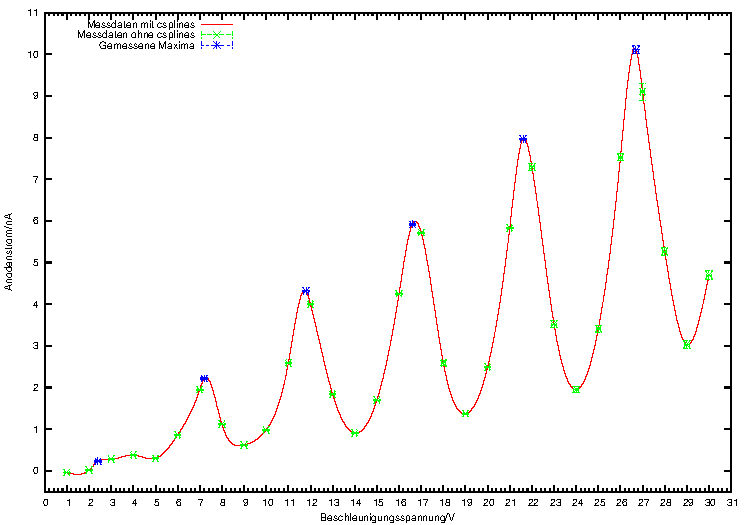
\includegraphics[scale= 1.5]{q_t.pdf}
	\caption{Graphische Darstellung des Anodenstroms in Abhängigkeit der Beschleunigungsspannung}
\end{figure}

Die Messdaten wurden mit csplines versehen, was kein physikalisches Modell darstellt sondern zu besseren Darstellung dient. Für den Plot wurden die Daten aus Tabelle \ref{tab:q_daten} und Tabelle \ref{tab:q__max_messung} verwendet.

Nach Gleichung \ref{eqn:kp} wurden die Kontaktpotentialdifferenz und nach Gleichung \ref{eqn:kp_delta} der Fehler bestimmt. Dabei ergab sich eine Wert von \unit[0,18 $\pm$ 0,33]{V}.

\subsection{Diskussion}
%es geht hier immer darum die gemessenen werte und die bestimmten werte über die messfehler mit literaturwerten oder untereiander zu vergleichen.
%dafür kann zu einen genannt werden, in welchem fehlerintervall des messwertes der literaturwert oder der vergleichswert liegt, und zum anderen der relative anteil des fehlers am messwert bestimmt, und damit die qualität unserer messung abgeschätzt werden.
%in einem satz soll dann kurz angesprochen werde, wie dut unser fehler und damit unsere messung also ist.
%nun sollte kurz angesprochen werden, wie systematische fehler unsere messung beeinflusst haben könnten.
%Zum schluss ist es wichtig anzusprechen, in wie weit die ergebnisse mit der theoretischen vorhersage übereinstimmen

Für die Anregungsspannung wurde ein Wert von \unit[4,9]{eV} erwartet,\footnote{Quelle: http://de.wikipedia.org/wiki/Franck-Hertz-Versuch aufgerufen am 22.09.2014 um 16:37 Uhr}, unser experimentell bestimmter Wert liegt bei \unit[4,86 $\pm$ 0,3]{eV}, dies entspricht einer Abweichung von 0,81\% was ein sehr guter Wert ist. Der Fehler ist in Relation zur prozentualen Abweichung groß, was an der Fehlerfortpflanzung der Mittelwertbildung liegt.

\section{Franck-Hertz Versuch für Neon}
%hier am besten kurz das ziel dieses versuchsteiles ansprechen, damit wir keine zwei überschriften übereinander haben!
%bei schwierigeren versuchen kann auch der theoretische hintergrund erläutert werden. (mit formeln, herleitungen und erklärungen)
Ziel der Messung ist es die Franck-Hertz-Kurve für Neon aufzunehmen und aus ihr die Energiedifferenz zwischen Grund- und angeregtem Zustand zu bestimmen, sowie die Kontaktpotentialdifferenz.

\subsection{Versuchsaufbau}
%skizze zum versuchsaufbau soll hier rein, foto geht auch aber es muss erklärt werden wie das ganze funktioniert und nochmal auf spezielle einstellungen eingegangen werden! z.b. welche knöpfe wir an unseren geräten für die messung verdreht haben.
\subsection{Versuchsdurchführung}
%hier soll hauptsächlich rein was wir machen, warum wir das machen und mit welchem ziel.
%es ist wichtig präzize zu erklären wie wir bei dem versuch vorgegangen sind und was wir tuen mussten.
Zuerst muss die Franck-Hertz Röhre (Neon) $\frac{U_2}{10}$ (Kanal 1 des Oszilloskops := X-Achse) und $U_A$ (Kanal 2 des Oszilloskops := Y-Achse) an das Oszilloskop angeschlossen werden und die Franck-Hertz Kurve mit der Sägezahnspannung konfiguriert werden. Dazu können die Saugspannung $U_1$ und die Bremsspannung $U_3$ am Franck-Hertz Betriebsgerät verdreht, sowie
am Oszilloskop die Auflösung in X- und Y-Richtung und die Verschiebung der Kurve auf der X- und Y-Achse eingestellt werden.
Sobald die Franck-Hertz Kurve am Oszilloskop gut zu erkennen ist, kann das Franck-Hertz Betriebsgerät auf den manuellen Modus umgestellt werden. Nun kann die Kurve von Hand durch verändern der Beschleunigungsspannung $U_2$ durchgefahren und einige Messerte aufgenommen werden. Danach werden zusätzlich die genauen Maxima ausgemessen um später die Anregungsspannung bzw. Anregungsenergie aus dem Mittelwert der Differenzspannungen $U_{\Delta}$ (zwischen zwei nebeneinander liegenden Maxima) zu bestimmen.
Zum Schluss wollen wir die Kontaktpotentialdifferenz zwischen Anode und Kathode bestimmen.
Die Beschleunigungsspannung bis zum ersten Maximum ist dafür gleichzusetzen mit der Anregungsspannung der Quecksilberatome und der Kontaktpotentialdifferenz zwischen Anode und Kathode.
\subsection{Verwendete Formeln}
%es kann eine legende angefertigt werden aber die selbstverständlichen buchstaben müssen nicht extra erklärt werden.
%hier kommen mit knappen erklärungen nur die verwendeten formeln, sowie die zugehörige Fehlerrechnung rein.
Es wurden für den Franck-Hertz Versuch mit Neon die gleichen Formeln verwendet wie für Quecksilberdampf. (vgl. Franck-Hertz Versuch für Quecksilber 3.3)
\subsection{Messergebnisse}
%hier werden die messwerte in !übersichtlichen! tabellen angegeben
%falls zu viele kleine tabellen entstehen ist es sinnoll eine große tabelle daraus zu machen
%anders herum müssen zu große tabellen mit dem [scale] befehl scaliert werden oder in zwei kleinere tabellen aufgeteilt werden.
%es ist wichtig vor !jeder! tabelle zu sagen, was gemessen wurde und wie wir unsere fehler gewäht haben. aber vor allem muss ausreichend !erklärt! werden, !warum! wir unsere fehler grade so gewählt haben.
\subsection{Auswertung}
%hier sollen zuerst !alle! errechneten werte entweder in ganzen Sätzen genannt, oder in tabellen(übersichtilicher) dargestellt, sowie auf die verwendeten formeln verwiesen werden. die referenzierung der formel kann in der überschrift stehen.
%es soll immer kurz erwähnt werden, warum wir das ganze ausrechnen bzw. was wir dor ausrechnen.
%danach werden histogramme und plots erstellt, wobei wenn möglich funktionen durch die plots gelegt werden sollten. (zur not können auch splines benutzt werden, was aber angesprochen werden muss)
%bei fits sollte immer die funktion und das reduzierte chiquadrat mit angegeben werden, wobei auf verständlichkeit beim entziffern der zehnerpotenzen geachtet werden sollte z.b. f(x)=(wert+-fehler)\cdot10^{irgendeine zahl}\cdot x + (wert+-fehler)\cdot10^{irgendeine zahl}
%es muss bei jedem fit erklärt werden, nach welchem zusammenhang gefittet wurde und warum!
%bei plots darauf achten, dass die achsenbeschriftung die richtige größe hat und die Legende im plot nicht die Messwerte verdeckt
%zusätzlich soll in diesem teil die aufgabenstellung abgehandelt werden.
\subsection{Diskussion}
%es geht hier immer darum die gemessenen werte und die bestimmten werte über die messfehler mit literaturwerten oder untereiander zu vergleichen.
%dafür kann zu einen genannt werden, in welchem fehlerintervall des messwertes der literaturwert oder der vergleichswert liegt, und zum anderen der relative anteil des fehlers am messwert bestimmt, und damit die qualität unserer messung abgeschätzt werden.
%in einem satz soll dann kurz angesprochen werde, wie dut unser fehler und damit unsere messung also ist.
%nun sollte kurz angesprochen werden, wie systematische fehler unsere messung beeinflusst haben könnten.
%Zum schluss ist es wichtig anzusprechen, in wie weit die ergebnisse mit der theoretischen vorhersage übereinstimmen
\section{Fazit}
%im fazit soll nochmal alles zusammengefasst werden und der verlauf der messung abgeschätzt werden
%gravierende sytematische probleme bei den messungen müssen nochmal betont und die wertigkeit unserer ergebnisse sollte nocheinmal eingeordnet werden.

\end{document}